\documentclass[russian, unicode, mathserif, aspectratio=169]{beamer}
% handout - to disable overlays

\usepackage{NeuroFuzzy}
\usepackage{amsmath}
\let\Sun\relax
\let\Moon\relax
\let\Mercury\relax
\let\Venus\relax
\let\Earth\relax
\let\Mars\relax
\let\Jupiter\relax
\let\Saturn\relax
\let\Uranus\relax
\let\Neptune\relax
\let\Pluto\relax
\let\Gemini\relax
\let\Leo\relax
\let\Libra\relax
\let\Scorpio\relax
\let\Aries\relax
\let\Taurus\relax
\let\bigplus\relax

\usepackage{mathabx}
\addbibresource{diploma.bib}
\title{Мера специфичности качественных распределений возможностей}
\author{Студент 435 группы\\ Ященко Михаил\,Андреевич\\Научный руководитель\\ к.ф-м.н Зубюк А.\,В.\\
% \footnotesize \href{http://NeuroFuzzy.phys.msu.ru}{http://NeuroFuzzy.phys.msu.ru},\\
% \href{mailto:fadeevegor@yandex.ru}{fadeevegor@yandex.ru},\\ \href{mailto:zubuk@cmpd2.phys.msu.ru}{zubuk@cmpd2.phys.msu.ru}
}
\institution{МГУ имени М.\,В.\;Ломоносова \\ Физический факультет \\ Кафедра математического моделирования и информатики}
\date{28 мая 2022\,г.}

\begin{document}
\selectlanguage{russian}
\sloppy

%%%%%%%%%%%%%%%%%%%%%%%%%%%%%%%%%%%%%%%%%%%%%%%%%%
% The title frame
%%%%%%%%%%%%%%%%%%%%%%%%%%%%%%%%%%%%%%%%%%%%%%%%%%
{
\usebackgroundtemplate{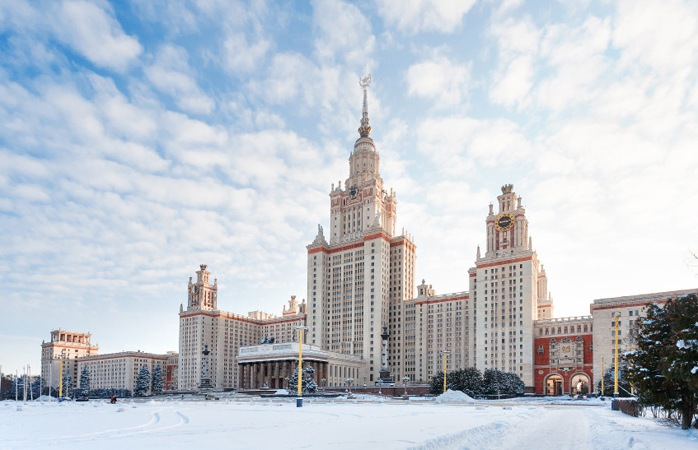
\includegraphics[width=\paperwidth, height=\paperheight]{msu-white}}
\maketitle
} 

%%%%%%%%%%%%%%%%%%%%%%%%%%%%%%%%%%%%%%%%%%%%%%%%%%
% Описание задачи
%%%%%%%%%%%%%%%%%%%%%%%%%%%%%%%%%%%%%%%%%%%%%%%%%%


\begin{frame}{Отношение специфичности ``$\preceq$''}
	
	\begin{itemize}
	    \item $\Omega = \{\omega_1, \omega_2, \ldots, \omega_n\}$,
	    \item распределение возможностей $\pi$ --- неотрицательная функция, $\underset{\omega \in \Omega}\sup\pi(\omega) = 1$, задающая упорядоченность на $\Omega$. 
	    \item $\Pi$ --- множество всех распределений возможностей на $\Omega$,
	    \item $\widetilde{\Pi} = \Pi \cup \{ \textbf{0} \}$,
	    \item $\pi_1, \pi_2 \in \widetilde{\Pi}$
	\end{itemize}
	\begin{definition}
	$\pi_1$ не менее специфично, чем $\pi_2$ ($\pi_1 \preceq \pi_2$), если
    \begin{itemize}
    \item $\supp \pi_1 \subset \supp \pi_2$,
    \item $\forall \omega_1, \omega_2 \in \supp \pi_1$, из $\pi_1(\omega_1) \leq \pi_1(\omega_2)$ следует $\pi_2(\omega_1) \leq \pi_2(\omega_2)$,
    \item $\forall \omega_1 \in \supp \pi_1$, $\forall \omega_2 \in \supp \pi_2 \backslash \supp \pi_1$, $\pi_2(\omega_1) \geq \pi_2(\omega_2)$.
    \end{itemize} 
	\end{definition}
	\justifying
	{\footnotesize
	\fullcite{zubyuk-fss-2018}
	}
\end{frame}

\begin{frame}{Супремум ``$\lor$'' и инфимум ``$\land$'' }
	
    \begin{definition}
    Супремум $\pi_1 \lor \pi_2$:
    \begin{itemize}
        \item $\pi_1 \preceq \pi_1 \lor \pi_2, \pi_2 \preceq \pi_1 \lor \pi_2$,
        \item $\forall \pi'$ таких, что $\pi_1 \preceq \pi'$ и $\pi_2 \preceq \pi'$: $\pi_1 \lor \pi_2 \preceq \pi'$
    \end{itemize}
    \end{definition}
    \begin{definition}
    Инфимум $\pi_1 \land \pi_2$:
    \begin{itemize}
        \item $\pi_1 \land \pi_2 \preceq \pi_1$, $\pi_1 \land \pi_2 \preceq \pi_2$,
        \item $\forall \pi'$ таких, что $\pi' \preceq \pi_1$ и $\pi' \preceq \pi_2$: $\pi' \preceq \pi_1 \land \pi_2$.
    \end{itemize}
    \end{definition}
	\justifying
	{\footnotesize
	\fullcite{ag-op-2021}
	}
\end{frame}

\begin{frame}{Решетка на классах эквивалентостей $(\widetilde{\Pi}, \preceq, \lor, \land)$}
    \begin{center}
	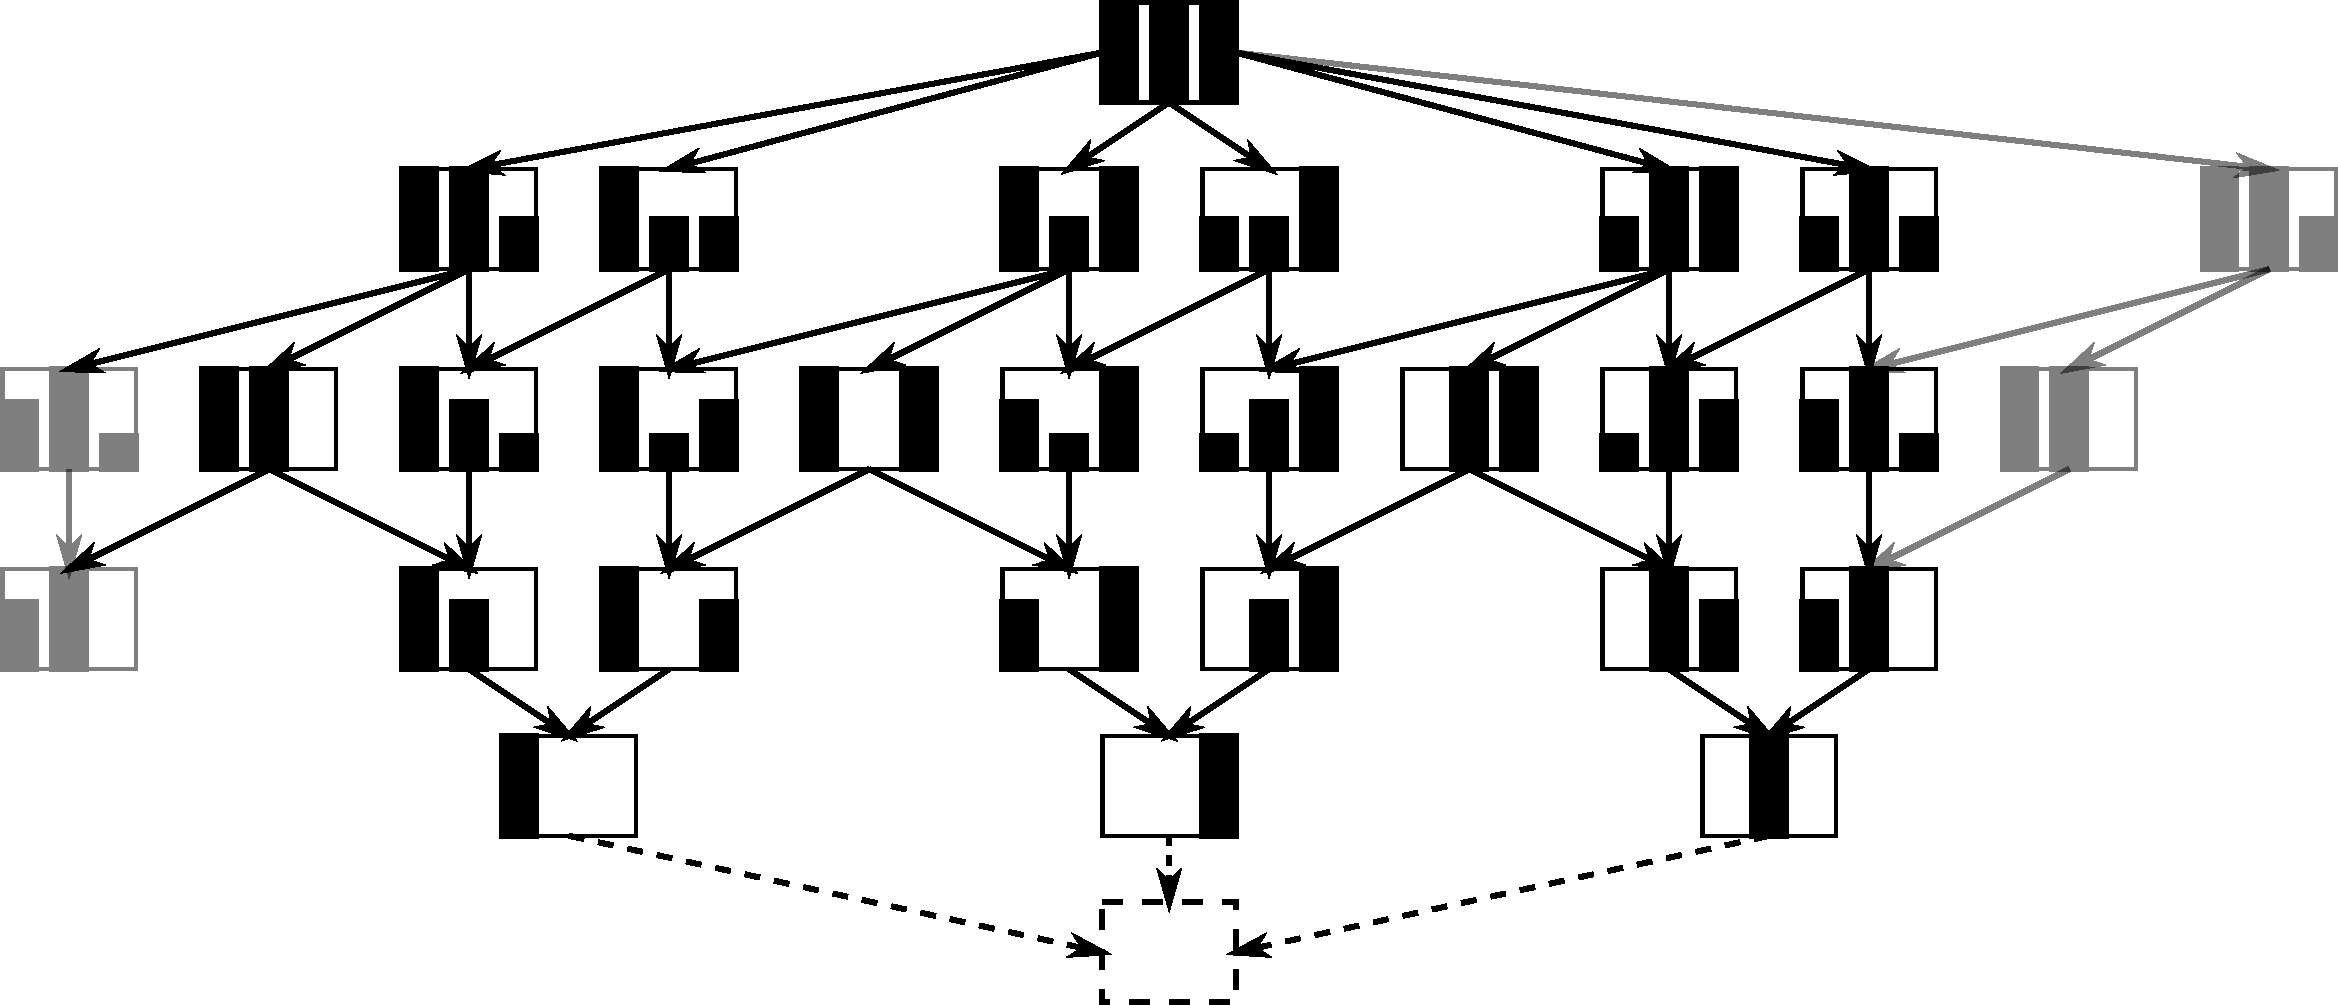
\includegraphics[width=0.6\textwidth]{pictures/three-point-omega.pdf}
	\end{center}
    Черные столбчатые диаграммы представляют все неэквивалентные распределения возможностей в случае $\Omega = \{\omega_1, \omega_2, \omega_3 \}$, $i$-ый столбей каждой диаграммы --- $\pi(\omega_i)$ в высоту. Любое другое распределение эквивалентно одному из распределений, показанных на рисунке. Стрелки демонстрируют отношение специфичности ``$\preceq$''. Они указывают от менее специфичных распределений к более специфичным. Столбчатые диаграммы, показанные серым цветом, являются дубликатами черных столбчатых диаграмм, они добавлены к рисунку, чтобы избежать стрелок, пересекающих его слева направо и наоборот. Пунктирный прямоугольник соответствует квазираспределению $\textbf{0}(\cdot) = 0$.
\end{frame}

%квазираспределение - самое специфичное

\begin{frame}{Задачи исследования}
    \begin{minipage}{0.5\textwidth}
    \begin{enumerate}
        \item
        \begin{itemize}
            \item $\pi_1, \pi_2 \in \widetilde{\Pi}$, $\pi_2 \preceq \pi_1$
            \item Разработать алгоритм нахождения расстояния $\rho(\pi_1, \pi_2)$ --- ?
        \end{itemize}
        \item
        \begin{itemize}
            \item $\pi_1$ --- мнение одного эксперта
            \item $\pi_2$ --- мнение второго эксперта\\
            $\pi_{\lor}=\pi_1 \lor \pi_2, \quad \pi_{\land} = \pi_1 \land \pi_2$
            \item Задать меру специфичности (меру согласованности) $\varphi(\pi_1, \pi_2)$
        \end{itemize}
    \end{enumerate}
    \end{minipage}
    \begin{minipage}{0.45\textwidth}
		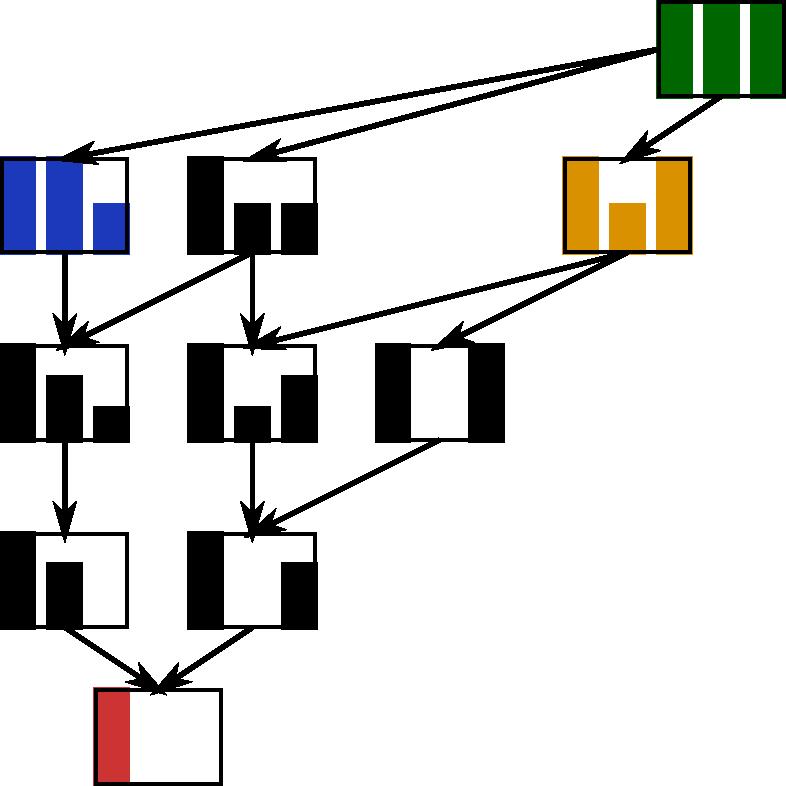
\includegraphics[width=\textwidth]{pictures/three-point-omega-example.pdf}
	\end{minipage}
\end{frame}

% \begin{frame}
% \textcolor{blue}{Алгоритм нахождения расстояния между распределениями}
% \end{frame}

% \begin{frame}{}
%   \centering \Large
%   \emph{\textcolor{blue}{Алгоритм нахождения расстояния между распределениями}}
% \end{frame}

\section{Алгоритм нахождения расстояния между распределениями}
{
\usebackgroundtemplate{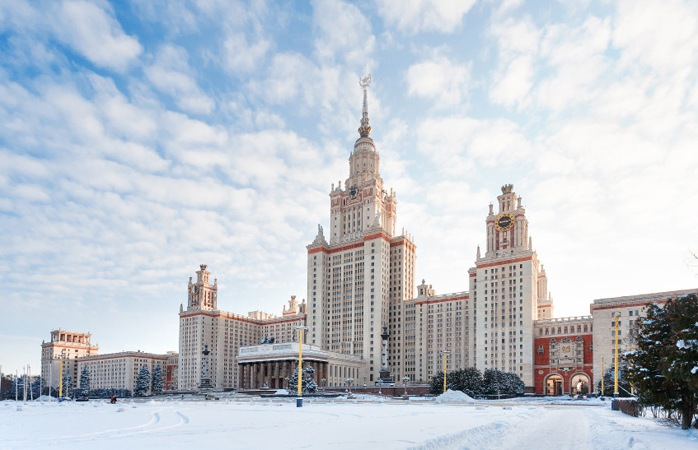
\includegraphics[width=\paperwidth, height=\paperheight]{msu-white}}
\frame{\transdissolve\sectionpage}
}

\begin{frame}{1-ый шаг алгоритма: Перестановка событий в $\pi_1$ и $\pi_2$}
    Переупорядочим события так, чтобы их возможности и в первом и во втором распределении были упорядочены по невозрастанию:
\begin{equation}
    1\rightarrow i_1, 2 \rightarrow i_2, \ldots, n \rightarrow i_n
\end{equation}
\begin{figure}[h!]
\center{
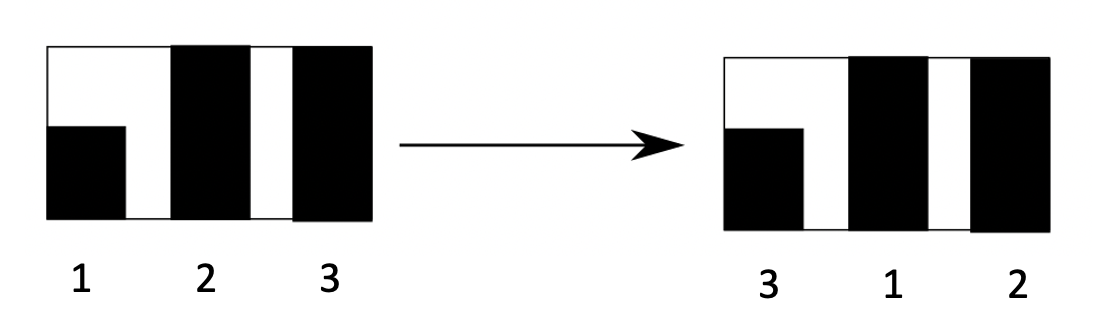
\includegraphics[width=210, height=70, scale=5]{pictures/image_11.png}
% \caption{Перестановка событий}
}
\end{figure}
\end{frame}

\begin{frame}{2-ой шаг алгоритма: Ставим каждому из распределений в соответствие двоичное число $e$}
    В теории возможностей Пытьева вводиться двоичное число $e \in (0,1)$, $e=0,e_1e_2\ldots e_n$,
которое определялось следующим образом:
\begin{equation}
    e_i =
      \begin{cases}
        1,    & \quad \text{если} \quad \pi(\omega_i) > \pi(\omega_{i+1})\\
        0,  & \quad \text{если } \quad \pi(\omega_i) = \pi(\omega_{i+1})
      \end{cases},\quad i = \overline{1, n-1}
\end{equation}
Расширим данное определение. Будем записывать в числе $e$ не только упорядоченности возможностей, но также, для наименьшей возможности, больше она или равна нулю. Это пригодится нам в дальнейшем.
\begin{equation}
    e_n =
      \begin{cases}
        1,    & \quad \text{если} \quad \pi(\omega_n) > 0\\
        0,  & \quad \text{если } \quad \pi(\omega_n) = 0
      \end{cases}
\end{equation}
Поставим распределениям $\pi_1$ и $\pi_2$ в соответствия числа $e_1$ и $e_2$:
$$\pi_1 \rightarrow e_{\pi_1},$$
$$\pi_2 \rightarrow e_{\pi_2}.$$
\end{frame}

\begin{frame}{Переход к 3-ему шагу алгоритма}
    \begin{minipage}{0.69\textwidth}
        \center{
		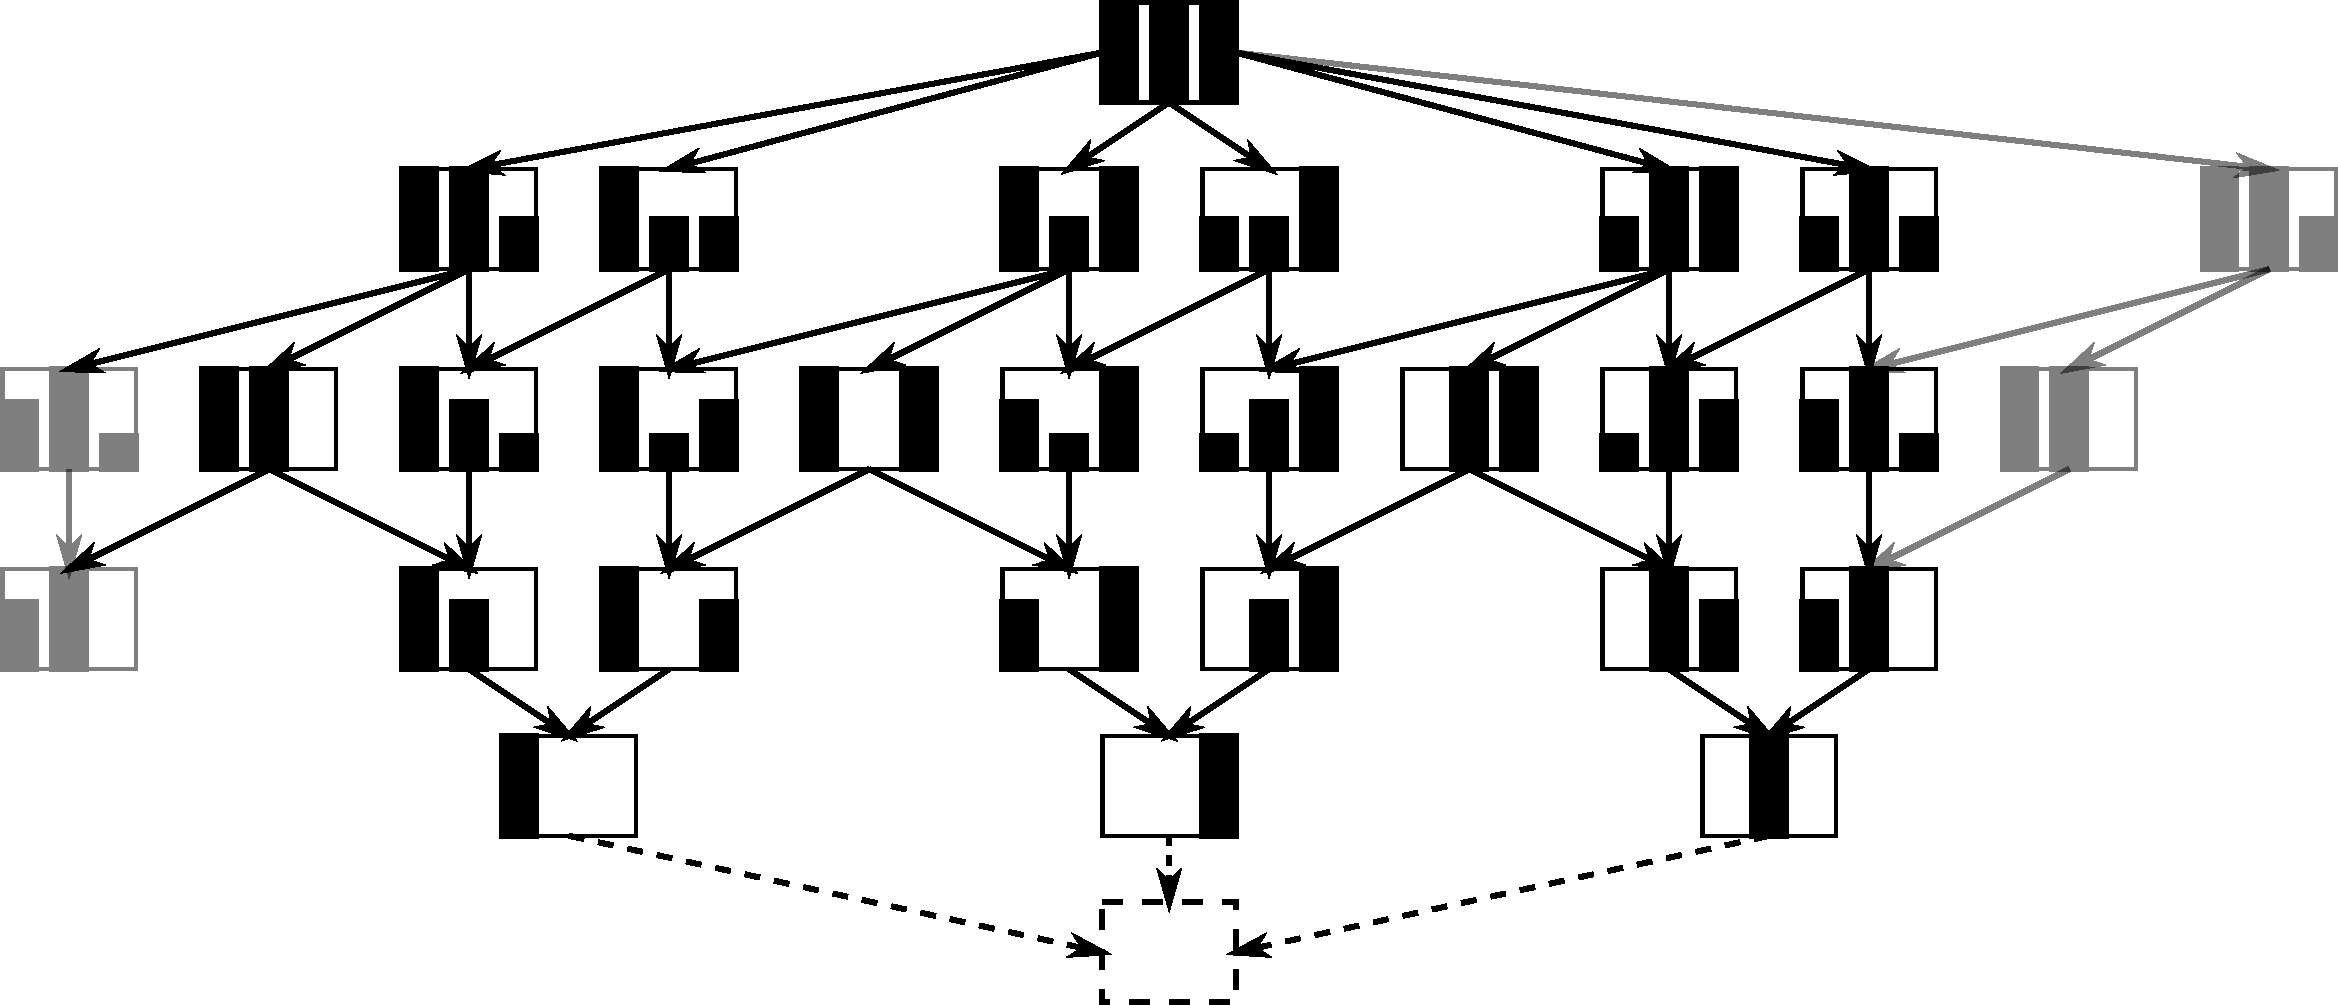
\includegraphics[width=\textwidth]{pictures/three-point-omega.pdf}
		\caption{Граф качественных распределений возможностей}
		}
	\end{minipage}
	   \begin{minipage}{0.2\textwidth}
        \center{
		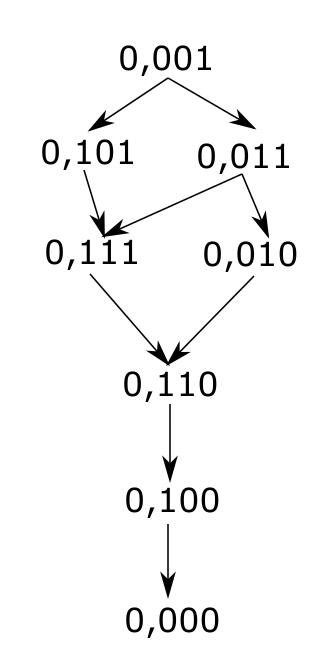
\includegraphics[width=\textwidth]{pictures/image_22b.png}
		\caption{Граф двоичных чисел $e$}
		}
	\end{minipage}
\end{frame}

\begin{frame}{3-ий шаг алгоритма: Построение графа доичных чисел $e$}
    \textbf{Ограничения при обходе}:
    \begin{enumerate} 
    \item Нули, которые стоят в конце числа e, не меняются $e=0,010\ldots1{\color{red}0\ldots0}$, так как это означает, что соответствующие возможности уже равны нулю, и их нельзя повысить, так как тогда нарушится отношение специфичности.
    \begin{figure}[h!]
    \center{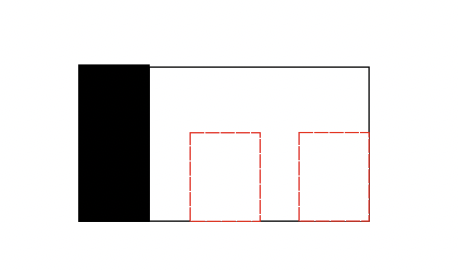
\includegraphics[width=90, height=45, scale=5]{pictures/image_2.png}}
    % \caption{Нули, которые стоят в конце числа e не меняются}
    \end{figure}
    \item $e=0,00{\color{red}0\ldots01} \nrightarrow e=0,00{\color{red}0\ldots00}$
    \begin{figure}[h!]
    \center{
\includegraphics[width=155, height=45, scale=5]{pictures/image_3.png}}
    % \caption{Невозможен переход от наименее специфичного распределению к наиболее специфичному}
    \end{figure}
    \end{enumerate}
\end{frame}

\begin{frame}{3-ий шаг алгоритма: Построение графа доичных чисел $e$}
    \textbf{Возможные действия при обходе:}
    \begin{enumerate}
        \item $e = 0,10\ldots1{\color{red}1}0\ldots0 \rightarrow e = 0,10\ldots1{\color{red}0}0\ldots0$
        \begin{figure}[h!]
            \center{
\includegraphics[width=103, height=33, scale=5]{pictures/image_4.png}}
        \end{figure}
        \item $e = 0,1{\color{red}0}0\ldots10\ldots0 \rightarrow e = 0,1{\color{red}1}0\ldots10\ldots0$\\
        $e = 0,10{\color{red}0}\ldots10\ldots0 \rightarrow e = 0,10{\color{red}1}\ldots10\ldots0$
        \begin{figure}[h!]
        \center{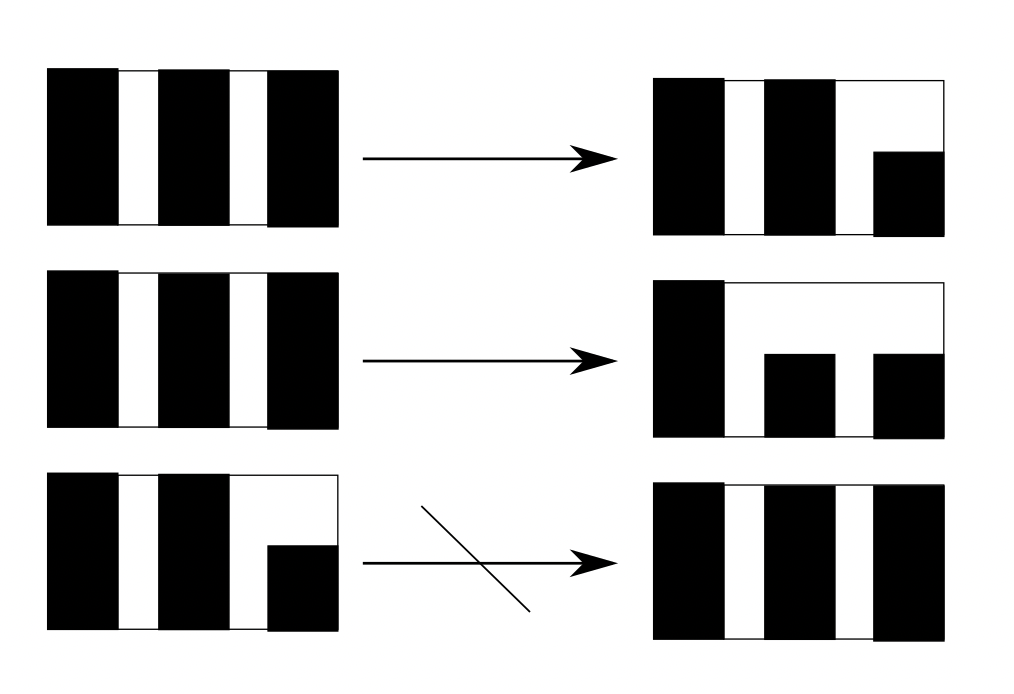
\includegraphics[width=103, height=100, scale=5]{pictures/image_5.png}}
        \end{figure} 
    \end{enumerate}
\end{frame}

\section{Определение меры специфичности}
{
\usebackgroundtemplate{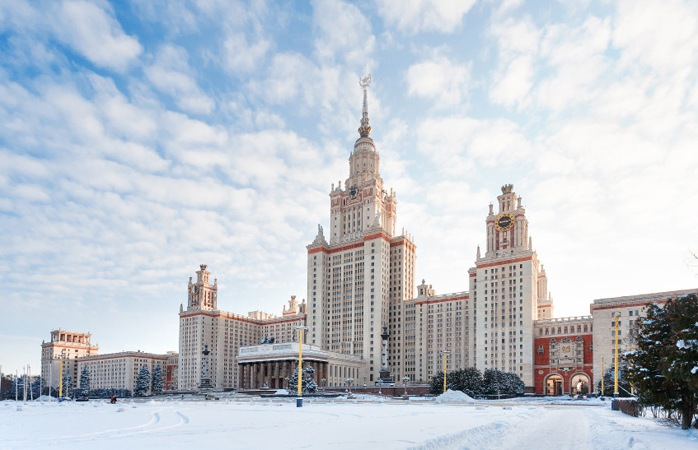
\includegraphics[width=\paperwidth, height=\paperheight]{msu-white}}
\frame{\transdissolve\sectionpage}
}

\begin{frame}{Мера специфичности}
\begin{equation}
    \varphi(\pi_1, \pi_2) = \frac{\rho_{max} - \rho(\pi_1 \lor \pi_2, \pi_1 \land \pi_2)}{\rho_{max}},
\end{equation}
где $\rho_{max} = 2n - 1$, так как расстояние между наименее специфичным и наиболее специфичным распределением равно $2n - 1$. Доказывается по индукции добавлением в $\Omega$ $\omega_{n+1}$.

Тогда, $\varphi(\pi_1, \pi_2) \in [0, 1]$, и чем больше $\varphi$, тем больше согласованы между собой экспертные оценки. Если $\varphi(\pi_1, \pi_2)$ маленькое, то экспертам не удалось договориться, и экспертные оценки рассогласованы.
\end{frame}

\begin{frame}{Примеры}
    \begin{center}
	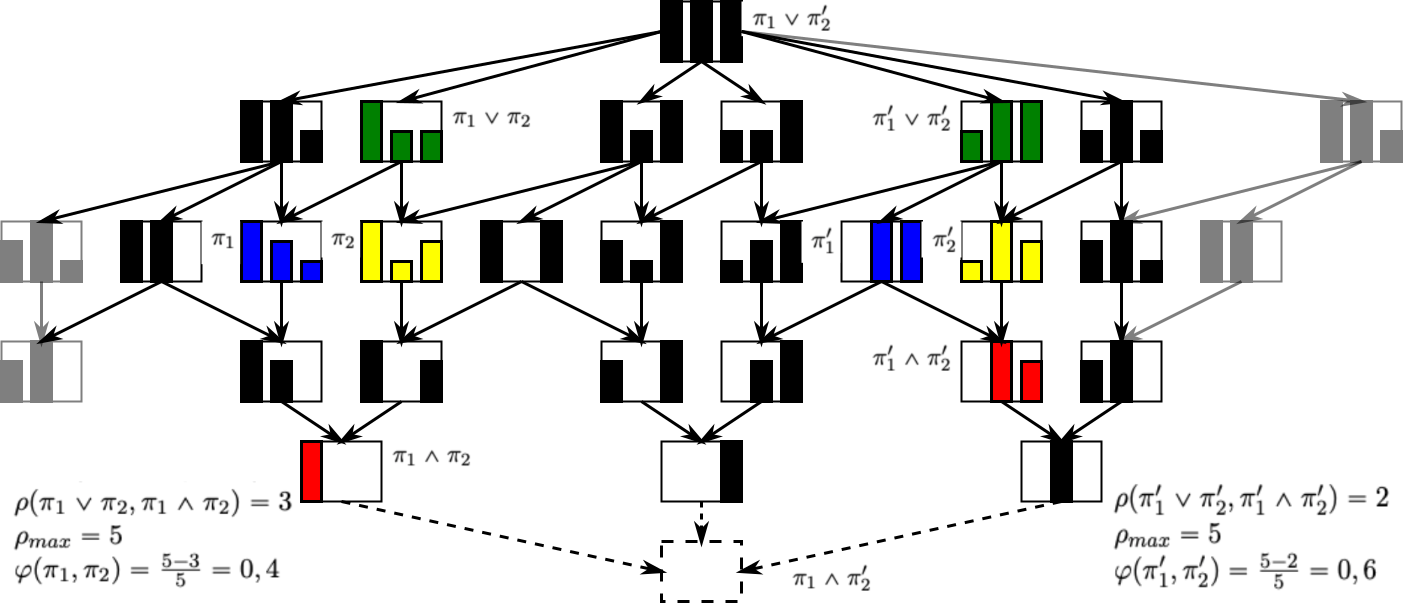
\includegraphics[width=0.97\textwidth]{pictures/three-point-omega-spec-examples.png}
	\end{center}
\end{frame}

\begin{frame}{Выводы}
    \begin{itemize}
        \item Был разработан алгоритм, который позволяет находить расстояние между двумя распределиями в графе качественных распределений возможностей
        \item Было сформулировано определение меры специфичности (меры согласованности), показывающей насколько согласованы между собой различные экспертные оценки.
    \end{itemize}
\end{frame}

\section{Спасибо за внимание!}
{
\usebackgroundtemplate{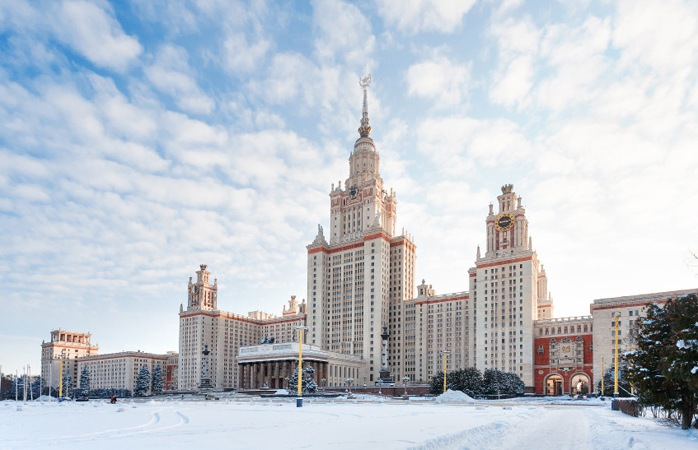
\includegraphics[width=\paperwidth, height=\paperheight]{msu-white}}
\frame{\transdissolve\sectionpage}
}

% \appendix
% \input{appendix.tex}

\end{document}

